\section{Mid-infrared grain emissivity}
\label{sec:grain-temp-emiss}

In preparation for our discussion of different wind mass-loss
diagnostic methods below, in this section we calculate the grain
emissivity predicted by models of dust heated by a nearby OB star.  We
use the same simulations that we employed in \S~4.2 of Paper~II,
% XREF: Paper II \ref{sec:cloudy-models-dust}
which employ the plasma physics code Cloudy \citep{Ferland:2013a,
  Ferland:2017a}.  In summary, simulations of spherically symmetric,
steady-state, constant density \hii{} regions were carried out for
four different stellar types from B1.5 to O5 (Table~2 of Paper~II), a
range of gas densities from \SIrange{1}{e4}{cm^{-3}}, and using
Cloudy's default ``ISM'' graphite/silicate dust mixture with 10 size
bins from \SIrange{0.005}{0.25}{\um}.  

\begin{figure}
  \centering
  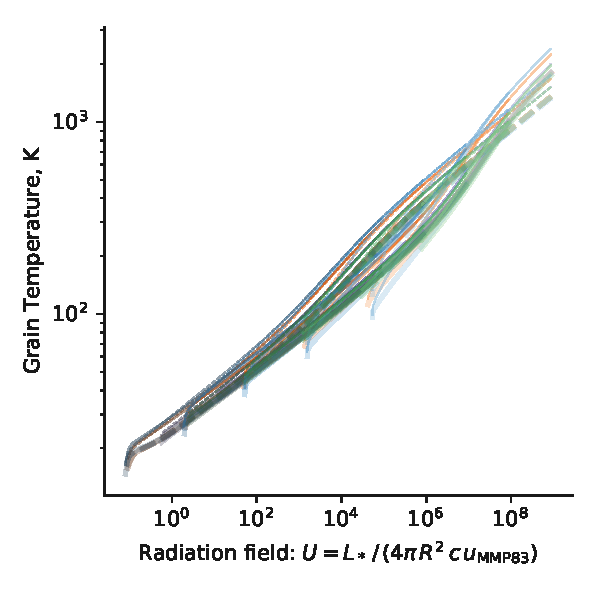
\includegraphics[width=\linewidth]{figs/grain-T-vs-U}
  \caption{Grain temperature versus radiation field mean intensity,
    \(U\), in units of the interstellar radiation field in the solar
    neighborhood.  Line types and colors correspond to a variety of
    stellar spectral shapes, gas densities, and grain species.  Dashed
    lines show carbon grains, solid lines show silicate grains, with
    line thickness and transparency increasing with grain size.
    Stellar spectral types are O5\,V (blue), O9\,V (orange), B1.5\,V
    (purple), and B0.7\,Ia (green), with lighter shades denoting
    higher gas densities. }
  \label{fig:grain-T-vs-U}
\end{figure}

Figure~\ref{fig:grain-T-vs-U} shows equilibrium grain temperatures for
these Cloudy models as a function of the nominal energy density of the
radiation field, \(U = u / u\mmp \), where \(u = L / 4 \pi R^2 c\) and
\(u\mmp\) is the energy density of the interstellar radiation field
for \(\lambda < \SI{8}{\um}\) in the solar neighborhood
\citep{Mathis:1983a}:
\begin{equation}
  \label{eq:u-mmp83}
  u\mmp\,c = \SI{0.0217}{erg.s^{-1}.cm^{-2}} \ .
\end{equation}
The tight relationship seen in Figure~\ref{fig:grain-T-vs-U} between
\(T\) and \(U\) is evidence for the dominance of stellar radiative
heating, which we justify on theoretical grounds in
\S~\ref{sec:unimp-other-heat} below.  The variation about the mean
relation is mainly due to differences in grain size and composition,
with smaller grains and graphite grains being relatively hotter.  The
downward hooks seen on the left end of each simulation's individual
curve are due to the fact that our calculation of \(U\) does not
account for internal absorption, which starts to become important near
the ionization front.

\begin{figure}
  \centering
  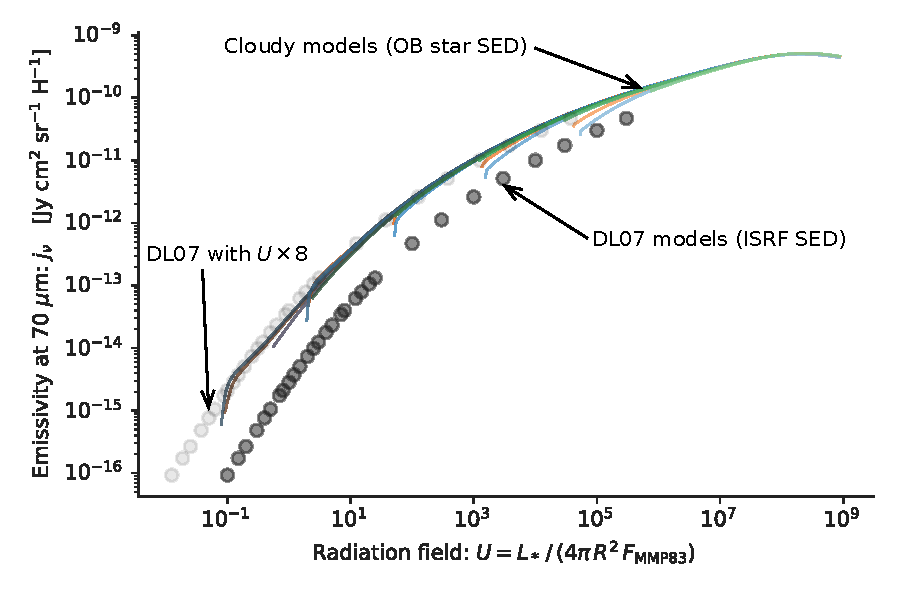
\includegraphics[width=\linewidth]{figs/grain-j70-vs-U-edited}
  \caption{Grain emissivity at \SI{70}{\um} for all Cloudy models,
    with lines colored as in Fig.~\ref{fig:grain-T-vs-U}, but without
    the variation in line type and thickness since emissivity is
    integrated over all grain types and sizes.  For comparison, the
    emissivity from the grain models of \citet{Draine:2007a} are shown
    as dark gray symbols, which assume illumination by a scaled
    interstellar radiation field with a SED with a very different
    shape from that of an OB star, see Fig.~\ref{fig:sed-comparison}.
    The light gray symbols show the effect of using an 8 times higher
    \(U\) with the \citeauthor{Draine:2007a} models, which
    approximately compensates for this difference in SED.  }
  \label{fig:grain-j70}
\end{figure}

The grain emissivity at \SI{70}{\um} (Herschel PACS blue band) for the
Cloudy simulations (colored lines) is shown in
Figure~\ref{fig:grain-j70}, where it is compared with the same
quantity from the grain models (dark gray symbols) of
\citet{Draine:2007a}.  A clear difference is seen between the two sets
of models, but this is due almost entirely to a difference in the
assumed spectrum of the illuminating radiation, as illustrated in
Figure~\ref{fig:sed-comparison}.  \citet{Draine:2007a} use a SED that
is typical of the interstellar radiation field in the Galaxy, which is
dominated by an old stellar population, which peaks in the near
infrared, with only a small FUV contribution from younger stars (about
8\% of the total energy density).  This is very different from the OB
star SEDs, which are dominated by the FUV and EUV bands.  Since the
grain absorption opacity is substantially higher at UV wavelengths
than in the visible/IR (see Fig.~6 of Paper~II),
% XREF: Paper II \ref{fig:cloudy-ism-dust-opacity}
the effective grain heating efficiency of the OB star SED is
correspondingly higher.  The light gray symbols show the effect on the
\citet{Draine:2007a} models of multiplying the radiation field by a
factor of \num{8} in order to offset this difference in efficiency,
which can be seen to bring them into close agreement with the Cloudy
models.  A further difference is that the \citet{Draine:2007a} model
includes small PAH particles, which we do not include in our Cloudy
models, since they are believed to be largely absent in photoionized
regions \citep{Giard:1994a, Lebouteiller:2011a}.  However, this only
effects the emissivity at shorter mid-infrared wavelengths
\(< \SI{20}{\um}\).

\begin{figure}
  \centering
  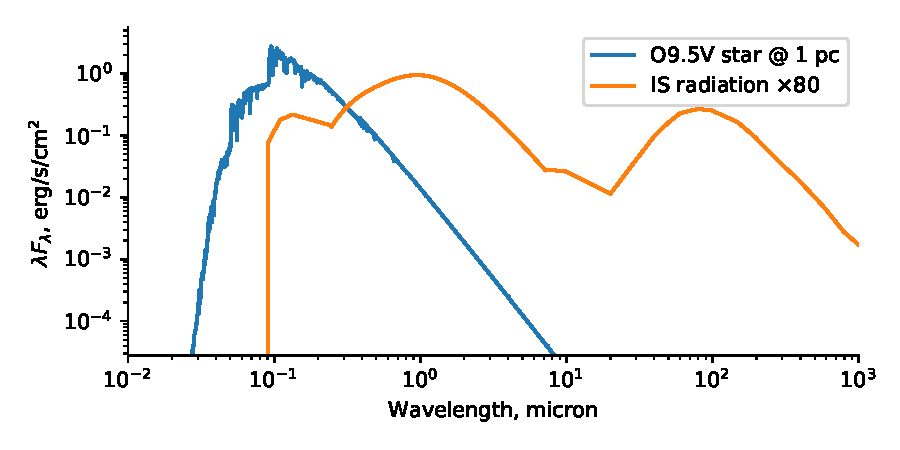
\includegraphics[width=\linewidth]{figs/sed-comparison}
  \caption{Comparison between the spectral energy distribution (SED)
    of a typical OB star (blue line) and the interstellar radiation
    field in the solar neighborhood (orange line).  The OB star is the
    \SI{20}{M_\odot} model from Table~1 of Paper~I and is plotted for
    a distance from the star of \SI{1}{pc}.  The interstellar SED is
    from \citet{Mathis:1983a} and is multiplied by \num{80} so that
    the total FUV-to-NIR flux is equal for the two SEDs.}
  \label{fig:sed-comparison}
\end{figure}

In terms of the characteristic parameters introduced in
\S~\ref{sec:energy-trapp-vers} the dimensionless radiation field
becomes
\begin{equation}
  \label{eq:U-from-L4-and-Rpc}
  U = 14.7\, L_4\, R_{\text{pc}}^{-2} \ ,
\end{equation}
or, alternatively, it can be expressed in terms of the ambient stream as
\begin{equation}
  \label{eq:U-from-ambient}
  U = 3.01 \, n \, v_{10}^2 / x^2 \ , 
\end{equation}
where \(x = R_0/R_*\) is given by Paper~I's equation~(12).
% XREF: Paper I \eqref{eq:x-cases}
It can also be related to the radiation parameter \(\Xi\), defined in
Paper~II's equation~(23), as
% XREF: Paper II \eqref{eq:Xi-Prad-over-Pgas}
\begin{equation}
  \label{eq:U-vs-Xi}
  U = 3.82 \, n T_4 \, \Xi \ .
\end{equation}
A common alternative approach to scaling the radiation field (see
\citealp{Tielens:1985a} and citations thereof) is to normalize in the
FUV band (\SIrange{0.0912}{0.24}{\um}), where the local interstellar
value is known as the Habing flux \citep{Habing:1968a}:
\begin{equation}
  \label{eq:Habing-flux}
  F\Hab = \SI{0.0016}{erg.s^{-1}.cm^{-2}} \ .
\end{equation}
The resultant dimensionless flux is often denoted by \(G_0\), and the
relationship between \(G_0\) and \(U\) depends on the fraction
\(f_{\text{fuv}}\) of the stellar luminosity that is emitted in the
FUV band:
\begin{equation}
  \label{eq:G-vs-U}
  G_0 = f_{\text{fuv}} \frac{u\mmp\, c}{F\Hab} \,U = (\text{\numrange{6}{10}}) \,U \ ,
\end{equation}
where we give the range corresponding to early O
(\(f_{\text{fuv}} \approx 0.4\)) to early B
(\(f_{\text{fuv}} \approx 0.7\)) stars, calculated from TLUSTY stellar
atmosphere models \citep{Lanz:2003a, Lanz:2007a}.

%% Single-photon heating of small grains

\subsection{Unimportance of other heating mechanisms}
\label{sec:unimp-other-heat}
The grain temperature in bows around OB stars is determined
principally by the steady-state equilibrium between the absorption of
stellar UV radiation (heating) and the thermal emission of infrared
radiation (cooling).  Other processes such as single-photon stochastic
heating, Lyman~\(\alpha\) line radiation, and post-shock collisional
heating can dominate in other contexts, but these are generally
unimportant for circumstellar bows, as we now demonstrate.

\subsubsection{Stochastic single-photon heating}
\label{sec:stoch-single-phot}
When the radiation field is sufficiently dilute, then a grain that
absorbs a photon has sufficient time to radiate all that energy away
before it absorbs another photon \citep{Duley:1973a}.  In this case,
the emitted infrared spectrum for \(\lambda < \SI{50}{\um}\) becomes
relatively insensitive of the energy density of the incident radiation
\citep{Draine:2001a}.  However, this is most important for the very
smallest grains.  From equation~(47) of \citet{Draine:2001a}, one
finds that grains with sizes larger than
\(a = \SI{0.005}{\um} = \SI{5}{nm}\) (the smallest size included in
our Cloudy models) should be close to thermal equilibrium for
\(U > 30\), which is small compared with typical bow shock values
(\(U = \text{\numrange{e3}{e6}}\)).  As mentioned above, PAHs are not
expected to be present in the interior of \hii{} regions.
\citealp{Desert:1990a} found them to be strongly depleted for
\(U > 100\) around O stars.  However, other types of ultra-small
grains, down to sub-nm sizes \citep{Xie:2018a} may be present in bows,
and stochastic heating \emph{would} be important for grains with
\(a = \SI{1}{nm}\) if \(U < \num{e5}\).  Note, however that grains
smaller than \SI{0.6}{nm} would be destroyed by sublimation after
absorbing a single He-ionizing photon.


\subsubsection{Lyman \(\alpha\) heating}

On the scale of an entire \hii{} region, the dust heating is typically
dominated by Lyman \(\alpha\) hydrogen recombination line photons, which
are trapped by resonant scattering (e.g., \citealp{Spitzer:1978a}
\S~9.1b).  However, this is no longer true on the much smaller scale
of typical bow shocks.  An upper limit on the Lyman \(\alpha\) energy
density can be found by assuming all line photons are ultimately
destroyed by dust absorption rather than escaping in the line wings
(e.g., \citealp{Henney:1998b}), which yields
\begin{equation}
  \label{eq:U-Lya}
  U\Lya \approx 0.1 n / \kappa_{600} \ .
\end{equation}
This can be combined with equation~\eqref{eq:U-from-ambient} to give
the ratio of Lyman \(\alpha\) to direct stellar radiation as
\begin{equation}
  \label{eq:Lya-over-stellar}
  \frac{U\Lya}{U} \approx 0.03 \frac{x^2}{v_{10}^2 \kappa_{600}} \ .
\end{equation}
Taking the most favorable parameters imaginable of a slow stream
(\(v_{10} = 2\)), very strong wind (\(x \approx 1\)), and reduced dust
opacity (\(\kappa_{600} = 0.1\)) gives a Lyman \(\alpha\) contribution of only
10\% of the stellar radiative energy density.  In any other
circumstances, the fraction would be even lower.

\subsubsection{Shock heating}
\newcommand\kin{\ensuremath{_{\text{kin}}}}
The outer shock thermalizes the kinetic energy of the ambient stream,
which may in principle contribute to the infrared emission of the bow.
In order for this process to be competitive, the following three
conditions must all hold:
\begin{enumerate}[1.]
\item The post-shock gas must radiate efficiently with a cooling
  length less than the bow size, see \S~3.2 of Paper~I.\@
  % XREF Paper I \ref{sec:radi-cool-lengths}
  This is satisfied for all but the lowest densities (Paper~I's
  Fig.~2).
  % XREF Paper I \ref{fig:zones-v-n-plane}
\item A significant fraction of the shock energy must be radiated by
  dust.  This requires that the post-shock temperature be greater than
  \SI{e6}{K}, which requires a stream velocity
  \(v_\infty > \SI{200}{km.s^{-1}}\) \citep{Draine:1981a}.  This also
  coincides with the range of shock velocities where the smaller
  grains will start to be destroyed by sputtering in the post-shock
  gas.
\item The kinetic energy flux through the shock must be significant,
  compared with the fraction of the stellar radiation flux that is
  absorbed and reprocessed by the bow shell.
\end{enumerate}
It turns out that the third condition is the most stringent, so we
will consider it in detail.  The kinetic energy flux through the outer shock for an ambient stream of density \(\rho_\infty\) and velocity \(v_\infty\) is
\begin{equation}
  \label{eq:Fkin}
  F\ke = \tfrac12 \rho_\infty v_\infty^3 = \tfrac12 P\shell v_\infty \ , 
\end{equation}
while the stellar radiative energy flux absorbed by the shell is
\begin{equation}
  \label{eq:Ftrap}
  F\trap \approx \tau L / 4 \pi R_0^2 \ ,
\end{equation}
assuming an absorption optical depth \(\tau \ll 1\). The shell
pressure in the WBS case can be equated to the ram pressure of the
internal stellar wind (see
% XREF Paper I \ref{sec:three-bow-regimes}
\S~2.1 of Paper~I), so that the ratio of the two energy fluxes is
\begin{equation}
  \label{eq:F-ratio-shock}
  \frac{F\ke}{F\trap} = \frac12 \frac{\eta\wind}{\tau} \frac{v_\infty}{c} \ .
\end{equation}
An upper limit to the stellar wind momentum efficiency \(\eta\wind\) is
the shell momentum efficiency \(\eta\shell\) that is derived
observationally in \S~\ref{sec:energy-trapp-vers}, where it is found
that \(\eta\shell / \tau < 30\) for all sources considered.  Therefore, for
a stream velocity \(v_\infty = \SI{200}{km.s^{-1}}\), we have
\(F\ke/F\trap < 0.01\) and the shock-excited dust emission is still
negligible.  Only in stars with \(v_\infty > \SI{1000}{km.s^{-1}}\) would
the shock emission start to be significant, and such hyper-velocity
stars \citep{Brown:2015a} do not show detectable bow shocks.

So far, we have only considered the outer shock, but the inner shock
that decelerates the stellar wind will have a velocity of
\SIrange{1000}{3000}{km.s^{-1}} and therefore might have a significant
kinetic energy flux by eq.~\eqref{eq:F-ratio-shock}.  However, the
stellar wind from hot stars will be free of dust,\footnote{%
  With the exception of Wolf-Rayet colliding wind binary systems
  \citep{Tuthill:1999a, Callingham:2019a}.} %
so that it would be necessary for the stellar wind protons to cross
the contact/tangential discontinuity and deposit their energy in the
dusty plasma of the shocked ambient stream in order for this source of
energy to contribute to the grain emission.  This is not possible
because the Larmor radius (see \S~5 of Paper~II)
% XREF Paper II \ref{sec:magn-effects-grain}
of a \SI{3000}{km.s^{-1}} proton in a \SI{1}{\micro G} field is only
\SI{3e10}{cm}, which is millions of times smaller than typical bow
sizes.  The magnetic field in the outer shell is unlikely to be
smaller than \(\approx n^{1/2} \si{\micro G}\), given that Alfvén speeds of
\SI{2}{km.s^{-1}} are typical of photoionized regions \citep{Arthur:2011a, Planck-Collaboration:2016c}
% XREF Paper II \\ref{eq:alfven}
and if the density were much lower than
\SI{1}{cm^{-3}}, then the scale of the bow would be commensurately
larger anyway.  Three-dimensional MHD simulations of bow shocks
\citep{Katushkina:2017a, Gvaramadze:2018a} show that the magnetic
field lines are always oriented parallel to the shell, so that high
energy particles from the stellar wind would be efficiently reflected
in a very thin layer and cannot contribute to grain heating.  For the
same reason, heat conduction by electrons across the contact
discontinuity is also greatly suppressed \citep{Meyer:2017a}.



%%% Local Variables:
%%% mode: latex
%%% TeX-master: "bs-bw-dw-03"
%%% End:
